\documentclass{standalone}
% translate with >> pdflatex -shell-escape <file>

% This file is an extract of the PGFPLOTS manual, copyright by Christian Feuersaenger.
% 
% Feel free to use it as long as you cite the pgfplots manual properly.
%
% See
%   http://pgfplots.sourceforge.net/pgfplots.pdf
% for the complete manual.
%
% Any required input files (for <plot table> or <plot file> or the table package) can be downloaded
% at
% http://www.ctan.org/tex-archive/graphics/pgf/contrib/pgfplots/doc/latex/
% and
% http://www.ctan.org/tex-archive/graphics/pgf/contrib/pgfplots/doc/latex/plotdata/

\usepackage{pgfplots}
\pgfplotsset{compat=newest}

\pagestyle{empty}

\begin{document}
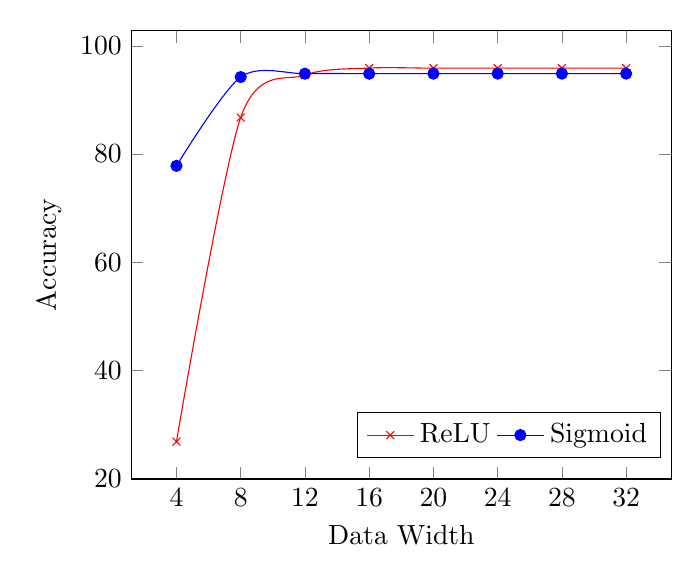
\begin{tikzpicture}
\begin{axis}[
	xlabel=Data Width,
	ylabel=Accuracy,
    legend style={at={(0.7,0.15)},
    anchor=north,legend columns=-1},
    xtick={0,4,8,12,16,20,24,28,32}]
\addplot[smooth,color=red,mark=x] coordinates {
	(4,   26.86)
	(8,   86.75)
	(12,  94.59)
	(16,  95.89)
	(20,  95.87)
	(24,  95.87)
	(28,  95.87)
	(32,  95.87)
};

\addplot[smooth,color=blue,mark=*] coordinates {
	(4,   77.82)
	(8,   94.23)
	(12,  94.85)
	(16,  94.85)
	(20,  94.86)
	(24,  94.86)
	(28,  94.86)
	(32,  94.86)
};

\legend{ReLU,Sigmoid}
\end{axis}
\end{tikzpicture}
\end{document}
